\documentclass[11pt]{article}
\usepackage{geometry} % see geometry.pdf on how to lay out the page. There's lots.
\usepackage{hyperref}
\usepackage{graphicx}
\usepackage{gensymb}
\usepackage[affil-it]{authblk}
\usepackage[toc,page]{appendix}
\usepackage{pifont}
\usepackage{amsmath}
\usepackage{amsthm}
\usepackage{amsfonts}

\usepackage{float}

\newtheorem{theorem}{Theorem}
\newtheorem{corollary}{Corollary}

\newcommand\numberthis{\addtocounter{equation}{1}\tag{\theequation}}


\usepackage{draftwatermark}



\SetWatermarkText{DRAFT}
\SetWatermarkScale{6}
\SetWatermarkLightness{0.95}

% \geometry{letter} % or letter or a5paper or ... etc
% \geometry{landscape} % rotated page geometry

% See the ``Article customise'' template for come common customisations

\title{Untwisting the Tetrahelix (v0.6)}
\author{Robert L. Read \texttt{read.robert@gmail.com} \and
  Robert Gatliff \texttt{robert@toubat.org}
}


\date{\today}

%%% BEGIN DOCUMENT
\begin{document}

\maketitle

%% \tableofcontents

\begin{abstract}
  The Boerdijk--Coxeter helix (BC helix, or tetrahelix) is a
  face-to-face stack of regular tetrahedra.  Considering the edges of
  these tetrahedra as structural members, the resulting structure is attractive and
  inherently rigid, and therefore interesting to architects,
  mechanical engineers, and robotocists.  A formula that matches the
  visually apparent helices forming the outer rails of the tetrahelix
  is derived which is convenient for designers.  This formula defines
  the vertices of tetrahelices of varying radius, pitch, and
  curvature, with the BC helix as a special case.  An addtional
  special case is of that of $0$ curvature or rail angle, which
  generates a \emph{tetrabeam}.  A particular choice of paramaters
  defines a novel object, the minimax optimal member length-difference
  tetrabeam, the \emph{equitetrabeam}.  A formula for computing the
  radius and z-axis travel that gives an optimal minimax tetrahelix
  for any rail angle between $0$ and $\rho_{bc}$ is given, thus
  defining a continuum of tetrahelices terminated by the equitetrabeam
  and BC helix. Numerically finding the rail angle from the equation for
  pitch allows optimal tetrahelices of any pitch to be designed.
  An interactive tool for such design and experimentation is provided.
  Utility and use for static and variable geometry
  truss/space frame design and robotics based on the are discussed.
\end{abstract}


\section{Introduction}

The Boerdijk--Coxeter helix\cite{coxeter1985simplicial} (BC helix), is
a face-to-face stack of tetrahedra that winds about a straight axis.
Because architects, structural engineers, and robotocists are inspired
by and follow such mathematical models but can build structures and
machines of differing or even dynamically changing length, it is
useful to develop the mathematics of structure formed from tetrahedra
where we relax regularity.


The vertices of the tetrahedra lie upon
three helices about the central axis.  The
Tetrobot/Glussbot\cite{TetrobotBook} project uses the regularity of
this geometry to make a tentacle-like robot that can crawl like a slug
or mollusc.  The Tetrobot concept is to use mechanical members, called
actuators, which can change their length, connected by special joints,
called the Song-Kwon-Kim\cite{song2003spherical} or turret joint,
which allow many members to come to a single point.  Such machines can
follow purely regular mathematical models such as the Boerdijk–-Coxeter
helix or the Octet Truss\cite{richard1961synergetic}.

Buckminster Fuller called the BC helix a \emph{tetrahelix}\cite{fuller1982synergetics},
a term now commonly used. In this paper we reserve \emph{BC helix} to mean the purely regular structre and use \emph{tetrahelix} to refer
to any structure isomophic to a the BC helix, whether regular or not.

\begin{figure}[H] %float with two figures
  \label{fig:closeup}
  \centering
     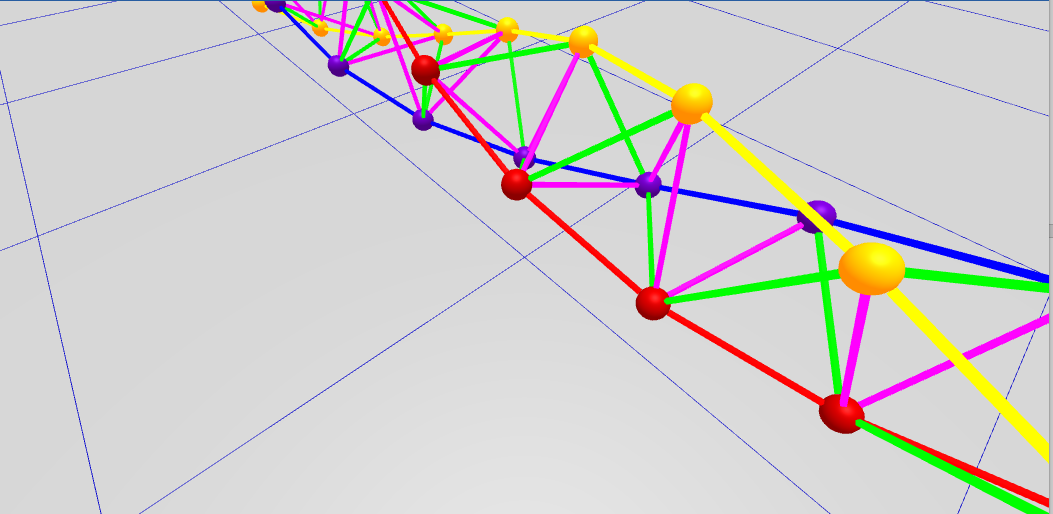
\includegraphics[width=0.95\textwidth]{figures/BCHelixCloseUp.png}
     \caption{BC Helix Close-up}
\end{figure}


Imagining Figure \ref{fig:closeup} as a static mechanical structure,
we observe that it is useful to the mechanical engineer or
robotocist because the structure remains an inherently rigid,
omni-triangulated space frame, which may be expected to be at least
somewhat mechanically strong.
Imagine further in Figure \ref{fig:closeup}, that each static edge was replaced with an
actuator that could dynamically become shorter or longer in response to electronic control,
and the they vertices were a joint that supported sufficient angular displacement
for this to be possible. Such a machine is a Tetrobot\cite{TetrobotBook}.

BC helix does not rest on a plane in a simple way. It is convenient to
be able to ``untwist'' it and to form a tetrahelix space frame that has a
flat planar surface. By making length changes in a certain way, we can
untwist a tetrahelix to form a \emph{tetrabeam} which has planar faces
and has, for example, an equilateral triangular profile. This paper
develops the equations needed to untwist the tetrahelix. All math
deveoped here is available in JavaScript and demonstrated by an interactive
design website\cite{readtetrahelix}, from which Figures \ref{fig:closeup} and
\ref{fig:series} are taken.

\begin{figure}[H] %float with two figures
  \label{fig:series}
  \centering
     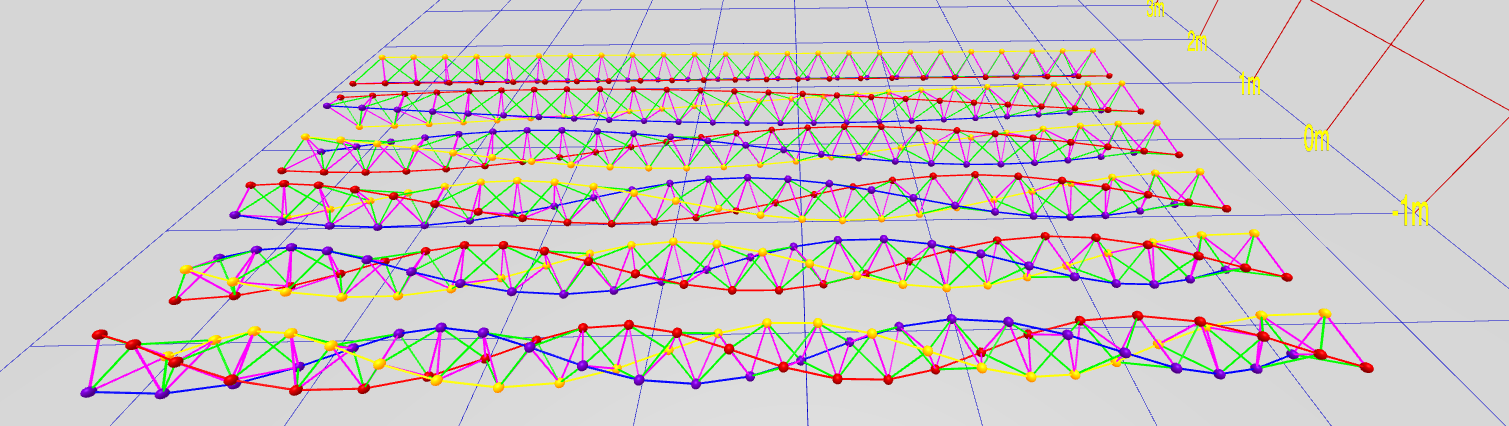
\includegraphics[width=0.95\textwidth]{figures/TetrahelixSeries.png}
     \caption{A Series of Tetrahelices, BC Helix in Foreground.}
\end{figure}

%% Note: This is not rendering figure two for some reason.
In Figure
\ref{fig:series}, the closest helix is the BC helix, and the furthest
is the equitetrabeam.

\section{A User's Formulation of the BC Helix}

If you can choose member lengths, you can form a linear combination of
the equitetrabream lengths and the completely regular lengths of the
tetrahelix, thereby choosing the amount of twist\footnote{The formal definiton
  of twistiness, or \emph{torsion}, is not useful or used in this paper, and
  we use \emph{curvature} without relying on the mathematical curvature easily
  computed from helical equations we provide.}.
If you are designing a
space frame, this is a static design choice, in a robot, it is a
dynamic choice that can be used to twist the robot and/or exert linear or
angular force on the environment.

Ideally we would have a simple formula for defining the nodes based on
any curvature or pitch we choose.  Unfortunately, it is not obvious that a linear
combination of lengths produces a simple formula.  It is a goal of
this paper to relate these two approaches to generating a tetrahelix
continuum.

H.S.M Coxeter constructs the BC helix\cite{coxeter1985simplicial} as a repeated rotation and translation of the tetrahedra, showing the
rotation is:
\[
\theta = \arccos(-2/3) 
\]
and the translation:
\[
h_{bc} = 1/\sqrt{10}
\]

$\theta$ is approximately $131.81$ degrees.
The angle $\theta$ is the rotation of a \emph{each} tetrahedra, not the tetraheda along a rail.  In Figure \ref{closeup},
each tetrahedra has either a yellow, blue, or red outer edge or rail.
That is, a blue-rail tetrahedron is rotated slightly more than a $1/3$ of a revolution to match the face of the yellow tetrahedra.

R.W. Gray's site\cite{graytetrahelix}, repeating a formula by Coxeter\cite{coxeter1985simplicial} in more accessible form, gives for a counter-clockwise BC Helix:
\begin{equation}
  \label{graycoxeter}
V(n) =
\left [
  \begin{tabular}{c}
   $ r_{bc} \cos(n \theta) $\\
   $ r_{bc} \sin(n \theta) $\\
   $ n h_{bc}  $
  \end{tabular}
  \right ],
\text{where:}
  \begin{tabular}{c}
 $ r_{bc} = \frac{3\sqrt{3}}{10} $\\
 $ h_{bc} = 1/\sqrt{10} $ \\
 $ \theta = \arccos(-2/3) $ \\
  \end{tabular}      
\end{equation}
where $n$ represents each integer numbered node in succession on every colored rail.

The apparent rotation of tetrhedra of the same outer-edge color ($V_3$ relative from $V_0$ for example,
in \eqref{graycoxeter}, is $3 \theta - 2\pi$.

This formula defines a helix, but it is not any of the apparent helices, or rail helices, of the
BC helix, but rather one that winds three times as rapidly through all
nodes. To a designer of tetrahelices, it is more natural to think of
the three helices which are visually apparent, that is, those three
which are closely approximated by the by the outer edges or rails of
the BC helix. We think of each of these three rails as being a different color, red, blue, or yellow.

It is convenient to have a formula that gives us the nodes of just
one rail helix, denoted by color $c$:
\[
(\forall n \in \mathbb{Z}, \forall c \in \{0,1,2\} : H_{BCcolored}(n,c) = V(3n +c))
\]

Such a helix can be written:
\begin{equation}
  \label{eq:colord}
H_{BCcolored}(n,c) =
\left [
  \begin{tabular}{c}
   $ r_{bc}  \cos((3 \theta - 2 \pi)n + c  \theta $\\
   $ r_{bc} \sin((3 \theta - 2 \pi)n + c  \theta $\\
   $ 3 h_{bc} (n + c/3)  $
  \end{tabular}
  \right ],
\text{where:}
  \begin{tabular}{c}
 $ r_{bc} = \frac{3\sqrt{3}}{10} $\\
 $ h_{bc} = 1/\sqrt{10} $ \\
 $ \theta = \arccos(-2/3) $ \\
  \end{tabular}      
\end{equation}

In this formula, integral values of $n$ may be taken as a node number for one rail and used to compute its Cartesian
coordinates. Allowing $n$ to take non-integer values defines a continuous
helix in space which is close to the segmented polyline of the outer tetrahedra edges, and coincides with them at integer
values.

The quantity $ (3 \theta - 2 \pi) \approx 35.43 \degree $, and is the angular shift between $V(3n+c)=H_{BCcolored}(n,c)$ and
$V(3(n+1)+c)=H_{BCcolored}(n+1,c)$.
This quantity appears so often that we call it the ``rail angle rho''. For the BC helix, $\rho_{bc} = (3 \theta - 2 \pi)$.

\begin{figure}[H]
  \label{railanglefig}
     \centering
     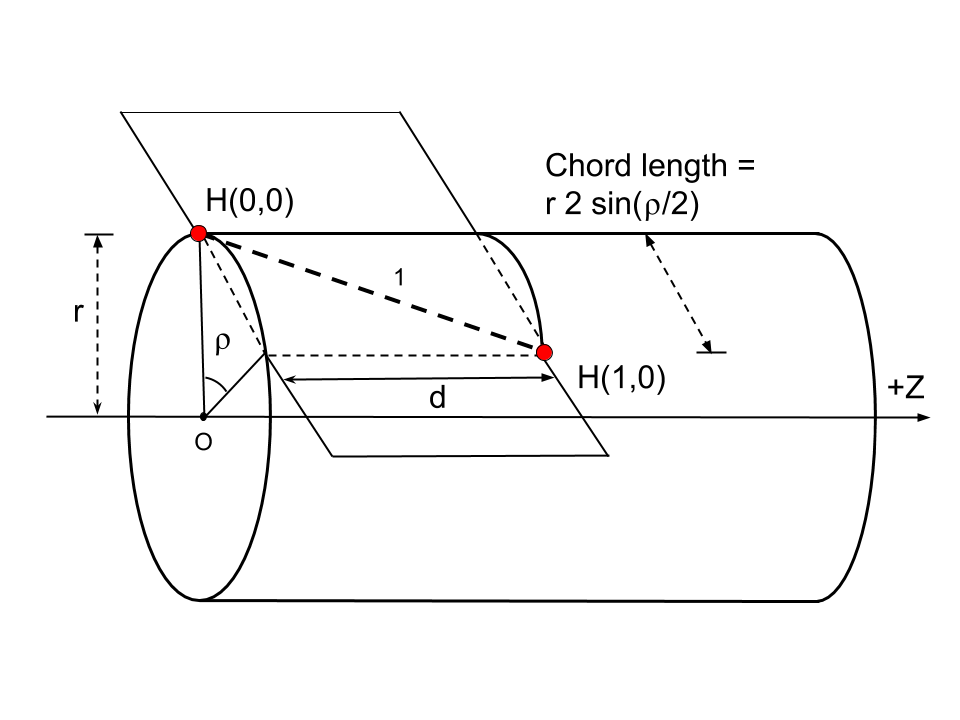
\includegraphics[width=0.7\textwidth]{figures/RailAngleGeometry.png}
     \caption{Rail Angle Geometry}
\end{figure}

Note in Figure \ref{railanglefig} the $z$-axis travel for one rail edge is denoted by $d$. In \eqref{graycoxeter} and \label{eq:colored}, the variable
$h$ is used for one third of the distance we name $d$. We will later justify that $d = 3h$. In this paper we assume the length of a rail
is alwyas $1$ is a simplification, although we make the rail length a parameter in our JavaScript codein \texttt{tetrahelixmath.js} \cite{readtetrahelix}.

Since:
\[ \frac{2 \pi}{\rho_{bc}} \approx 10.16
\]
We can see that there are approximately $10.16$ red, blue or yellow tetrahedra on one rail in a single revolution.
The pitch of the Boerdijk--Coxeter helix of edge length $1$ is the length of three tetrahedra times this number:
\begin{align*}
  &= \frac{d_{bc} 2 \pi }{\rho_{bc}} \\  
  &= \frac{3 \cdot h_{bc} 2 \pi }{\rho_{bc}} \\
  &= \frac{3  \sqrt{\frac{2}{5}}  \pi}{\rho_{bc}} \\
  &\approx 9.64 \\
\end{align*}
The pitch is less than the number of tetrahedra because the tetrahedra
are not lined up perfectly.  It is a famous and interesting result
that the pitch is irrational, a BC helix never has two tetrahedra at
precisely the same orientation around the $z$-axis. However, this is
inconvenient to designers, who might prefer a rational pitch.
The idea of deveoping a rational period by arranging solid tetrahedra by relaxing the face-to-face matching
has been explored\cite{sadler2013periodic}. In this paper
we develop slightly irregular edge lengths that support, for example, a pitch of precisely 10
tetrahedra in one revolution which would allow an architect to design a
column having a basis and a capital in the same relation to the
tetrahedra they touch at the bottom and top of the column.


\section{Optimal Tetrahelices Have $z$-axis Evenly Spaced Vertices}

We use the term \emph{tetrahelix} to mean any structure made of
vertices and edges which is isomorphic to the BC helix, in which the
vertices lie on three helices. We further demand that all edge lengths
be finite, as we are only interested in physically constructable tetrahelices.
By isomporphic we mean there is a one-to-one mapping between both
vertices and edges in the two tetrahelices.
One could consider various definitions of optimality for a
tetrahelix, but the must useful to an enginner is to minimize the
maximum difference between any two edges.

If all three rails do not have the same pitch, there is an edge of
unbounded length, so it is not optimal. So we are justified in talking about the
\emph{pitch} of 
the tetrahelix as the pitch of its rail helices, even though there are
three such helices.

Similarly, if the axes are not parallel, there is an edge of
unbounded length in the structure, so we exclude such a strcturue.

Since the axes are parallel, we may define the \emph{inradius} of a tetrahelix to be the radius of the largest
``in cylinder'': a
cylinder parallel to this axis contained within circumscribing cylinder which is penetrated by no edge.
Define an \emph{minimax edge-length optimal tetrahelix} or just an
\emph{optimal tetrahelix} to be a tetrahelix for which there exists
no other tetrahelix of the same inradius and pitch with a lower maximum
difference between its edge lengths. 

We wish to show that in an optimal tetrahelix, all vertices lie on the cylinder
of radius $r$, regardless of where they lie on the $z$-axis.

Since all three rails have the same rail length, no matter how we
move the rails in the $xy$ plane if we shorten the $xy$ distance between
vertices we shorten the total distance.
Our tool for thinking about this is to project out the $z$ dimension to form
a two-dimensional figure of nodes and non-rail edges.
Consider the projection along the $z$ axis of all vertices and non-rail edges into the $xy$ plane, which will be
a figure of dots and connecting segments in the $xy$ plane. The convex
hull for any one helix projection will be a circle (if its pitch is
irrational) or an polygon if rational, or a point if the helix has
zero curvature. Each of these figures by definitions lies outside the
circle of radius $r$ in the $xy$ plane.

\begin{theorem}
  Any optimal tetrahelix has all vertices on a single cylinder.
\end{theorem}

\begin{proof}



Case 1: Suppose that $\rho$ is zero. Then for any given inradius, an equilateral
triangle is the minimax solution for all non-rail edges. Since there is only
one rail-edge length, this is the minimax solution for the entire set. Since
the projection is an equilateral triangle lies on a circle, all points lie on
a cylinder.

Case 2: Suppose that $\rho$ is positive but less than $\pi$.
In this case each rail helix has
curavature and places points on both sides of any line through the origin
of the $xy$ plane (or both coincident on such a line.)

We first show that the inradius is touched by one segment from each pair
of rails.

\begin{figure}[H]
  \label{untouchingrailfig}
     \centering
     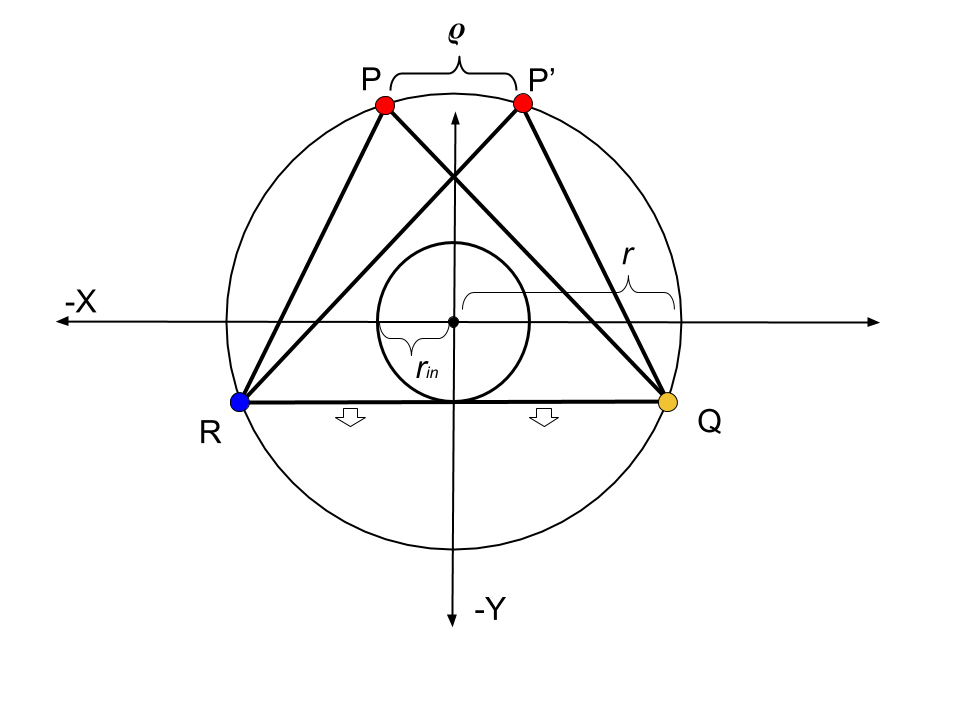
\includegraphics[width=0.7\textwidth]{figures/UntouchingRail.png}
     \caption{Untouching Rail}
\end{figure}

Figure\ref{untouchingrailfig} depicts a projection of
depicting only the point $P$, the point $P'$ which is an adjacent vertex on the same rail,
and the intermediary points $R$ and $Q$ on the other two rails.

Supoose there is a rail $P$ which does not have a segment touching the incircle
at all in the projection, as depicted in 
Then a segment connecting the other two $Q$ and $R$ is a longest
rail, because any chord touching an incircle is longer than any which does not.
These two rails ($Q$ and $R$) can be moved closer to each other, and further away from $P$, to form a better minimax solution
by shortening the longest rail, until one of the segments from $P$ the previously
untouching rail touches one of the incircle. By induction then all rails have
at least one segement touch each vertex on the rail that is tangent to the
the inradius in an optimal tetrahelix.

Now suppose that you attempt to move the axis of one of the rails. Because
$\rho > 0 $ and $\rho$ is not a multiple of $\pi$, there is some vertex on the two sides of any diameter
halving our circle. Moving the axis of a tetrahelix lengthens a longest line while ``pinching'' the
inradius on the other side, so it is not optimal. Since the axes of these helices are the
same and they have the same curvature and pitch, the points defined by the helices all lie
on a cylinder.


\end{proof}

Now that we have show that any optimal tetrahelix vertices that
are on helices of the same axes and pitch, we see that the vertices 
of any optimal tetrahelix will lie on a cylinder, or a circle when axis dimension
is projected out. Therefore is is reasonable to now speak of the \emph{radius}
of a tetrahelix as the radius of the cylinder, and the notion
of the projected incircle radius is now obsolete.

Now that we have coincident axes, the same pitch, we can go on to
 the hard proof about where they occur along the $z$-axis.

 We show that in fact the nodes must be distributed in even thirds
 along the $z$-axis.

 Note that from the point of view of a single edge, we are on a
 slanted cylinder, when $\rho \neq 0$.  This means for its point of
 view a cross section is an ellipse. So we have to be very careful in
 comparing lengths of edges relative to the tetrahedron, because a
 change in position along the edge changes the length of a line, but
 in a complicated way depending on where it is relative to the
 ellipse.

 In principle in any 3 helices with the same axis of the same radius
 having any relative
 displacement along the $z$ axis there are 9 distinct edge classes.
 If when projecting all vertices on the the $z$-axis, the interval
 defined by the $z$ axis value of its endpoints contains no other vertices,
 we call it a \emph{one-hop} edge, and if it does contain another vertex we
 call it a \emph{two-hop} edge.
 Then there are 
 3 rail edges, 3 one-hop lengths between each pair of 3 rails, and 3 two hop
 lengths between each pair of three rails, where the two-hop length is at least
 the one-hop length.
 However, we have already shown the rail
 lengths are equal in any optimal tetrahelix.

\begin{theorem}
   \label{eventhirds}
   A tetrahelix of a given radius and axial distance $d$ in which all nodes are evenly spaced at $d/3$ intervals on the $z$ axis is optimal.
     Any one tetrahedron in a tetrahelix has $1$ rail edge, $2$ one-hop edges connected to the rail and $2$ two-hop edges connected to the rail.
  The edge opposite of the rail edge is a one-hop edge.
\end{theorem}

\begin{proof}
    Consider the tetrahelix in which the vertices are evenly spaced at
    $h/3$ intervals on the $z$ axis. Every edge is either a rail edge,
    or it makes one hop, or it makes two hops. All of the one-hop
    edges are equal length.  All of the two-hop edges are equal
    length.
    
    Any displacemnt along the $z$ axis of any rail increases the
    length of one or two two-hop edges and shortens the length of one
    or two one-hop edges.  This increases the minimax distance no
    matter what the rail edge length is, since all rail edges are the
    same length. Therefore, an evenly spaced tetrahelix is the unique
    optimal for any given radius and height.
\end{proof}
  

 Note that based on \ref{eventhirds}, there are only 3 possible lengths in an optimal tethrahelix,
 and we are justified in classifying edge lengths as \emph{rail},\emph{one-hop}, or
\emph{two-hop}. The one-hop edges are the edges between closest on the $z$-axis, and the two-hop edges are those that hop over a vertex.

By Theorem \ref{eventhirds} every optimal tetrahelix has vertices lying on helices expressible in the form:
\[
V_{optimal}(n,c) =
\left [
  \begin{tabular}{c}
   $ r \cos(n \alpha +  c 2 \pi /3)$\\
   $ r \sin(n \alpha +  c 2 \pi /3) $\\
   $ \frac{d(n +c / 3)}{3}   $
  \end{tabular}
  \right ],
\text{where:}
\begin{tabular}{c}
  $c \in \{0,1,2\}$
  \end{tabular}      
\]
where we have not yet investigated in the general case the relationships beteween $\alpha$, $r$, and $d$ in this formulation.
However, we understand that when $\alpha = 0$, the helices are degenerate, having curvature of $0$, and
we have the equitetrabeam.


This formulation $V(n,c)$ above is valuable, but obscures the essentially fact that the red, yellow, and blue helices distributed
about the central $z$ axis $120\degree$ from each other.
In order to rewrite this expression with an explicit rotation of $2\pi/3$, we expand 
the expression and seek to isolate the term $c2\pi/3$.
\begin{align*}
  \rho_{bc} n + c \theta  &=   \text{\{we aim for 3 in denominator, so we split...\}} \\
    (3 \theta - 2 \pi)n + (c/3)  (3 \theta)  &=   \text{\{we want $2\pi$ in numerator, so add canceling terms...\}} \\
  (3 \theta - 2 \pi)n + (c/ 3) (3 \theta - 2 \pi  + 2 \pi) &=  \text{\{associate...\}} \\
  (3 \theta - 2 \pi)n + (c/ 3) ((3 \theta - 2 \pi)  + 2 \pi) &=  \text{\{distribute...\}} \\  
  (3 \theta - 2 \pi)n + (c / 3) (3 \theta - 2 \pi)  + c 2 \pi /3 &=  \text{\{definition of $\rho_{bc}$...\}} \\
  \rho_{bc} n + (c / 3) \rho_{bc}  + c 2 \pi /3 &=  \text{\{collect like factors...\}} \\  
  \rho_{bc} (n + c/3)  + c 2 \pi /3  \\
\end{align*}
Now the the term on the left is the only one that depends on the scalar $n$. We use this to a create
a new formulation: $H_{BCsymmetric}(n,c) = H_{BCcolored}(n,c)$

The expression $n+c/3$ will now occur so often that we call it the ``c($\kappa$)olored number'' and we use the variable $\kappa$ to represent it: $\kappa = n+c/3$.
Recall that $c \in \{0,1,2\}$, but $n$ and $\kappa$ are are continuous (rational or real-valued.)

\begin{equation}
H_{BCsymmmetric}(n,c) =
\left [
  \begin{tabular}{c}
   $ r  \cos(\rho_{bc} \kappa  + c 2 \pi /3) $\\
   $ r  \sin(\rho_{bc} \kappa  + c 2 \pi /3) $\\
   $ \kappa 3  h_{bc} $
  \end{tabular}
  \right ],
\text{where:}
  \begin{tabular}{c}
 $\kappa = n + c/3$ \\
    $\rho_{bc} = (3 \theta - 2 \pi)$ \\
    $ \theta = \arccos(-2/3) $ \\
    $ h_{bc} = 1/\sqrt{10} $ \\    
  \end{tabular}      
\end{equation}



\section{Parameterizing Tetrahelices via Rail Angle}

We seek a formula to generate optimal tetrahelices that accepts a
parameter that allows us to design the tetrahelix conveniently.
Please refer back to Figure \ref{railanglefig}.
The pitch of the helix is an obious choice, but is not defined when the
curvature is $0$, an important special case. The radius or the axial
distance between two nodes on the same rail are obvious choices, but
perhaps the clearest choice is to build formula that takes as its
input the ``rail angle'' $\rho$. We define $\rho$ to be the angle
formed in the X,Y plane $\angle A O B$ projecting out the $z$
axis and sighting along the positive $z$ axis. In other words, $\rho$
controls how far a rail edge of a tetrahelix deviates from being
parallel with the axis, or the ``twistiness'' of tetrahelix. We use
the parameter $\chi = 1$ to indicate a chirality or counter-clockwise,
and $\chi = -1$ for clockwise.



 These quantities are related by the expression:

\begin{align*}
  1^2 &= d^2 + (2 r \sin{ \rho / 2})^2 \\
  1 &= d^2 + 4 r^2 (\sin{ \rho / 2})^2 \\
  d^2 &= 1 - 4 r^2 (\sin{ \rho / 2})^2    \numberthis  \label{railangle} \\
\end{align*}

Checking the important special case of the BC helix, we find that this equation
indeed holds true (treating $d$ in this equation as $3 h_{bc}$ as defined by
Gray and Coxeter, that is, $d_{bc} = 3h_{bc}$, where they are using it for the axial height from one node to
the next of a different color, but we use it to mean distance for the same color.

The rail angle $\rho$ also has the meaning that $2 \pi / \rho$ is the number of
tetraheda in a full revolution of the helix.

In choosing $\rho$, one greatly constrains $r$ and $d$, but does not completely
determine both of them together, so we treat both as parameters.

Rewriting our formulation in terms of $\rho$:
\begin{equation}
  \label{eq:general}
H_{general}(\chi,n,c,\rho,d_{\rho},r_{\rho}) =
\left [
  \begin{tabular}{c}
   $ r_{\rho} \cos(\chi \cdot (\rho \kappa + c 2 \pi /3)) $\\
   $ r_{\rho}  \sin(\chi \cdot (\rho \kappa + c 2 \pi /3)) $\\
   $ d_{\rho} \kappa $
  \end{tabular}
  \right ],
\text{where:}
\begin{tabular}{c}
  $   1 = d_{\rho}^2 + 4 r_{\rho}^2 (\sin{ \rho / 2})^2 $ \\
  $\kappa = n + c/3$ \\
    $\chi \in \{-1,1\}$ \\  
  \end{tabular}      
\end{equation}


$H_{general}$ forces the user to select an $d_{\rho}$
which has a sensible radius.

Note that when $\rho = 0$ then $h_{\rho} = 1$, but $r_{\rho}$ is not determined by
Equation \ref{railangle}.

\begin{theorem}
  \label{generalformulaoptimal}
  The tetrahelices generated by $H_{general}$ are optimal in terms of minimum maximum member length when $r_{\rho}$ is chosen so that
  the length of the one-hop edge is equal to the rail length.
\end{theorem}


\begin{proof}
This is proved by a minimax argument.

By Theoerm \ref{eventhirds}, we can compute the (at most) three edge-lengths of an optimal
tetrahelix by (where $dist$ is the cartesian distance function):
\begin{align*}
  \text{rail} &= dist(H_{general}(n,c,\rho,d_{\rho},r_{\rho}),H_{general}(n+1,c,\rho,d_{\rho}),r_{\rho})) = 1 \\
  \text{one-hop} &= dist(H_{general}(n,c,\rho,d_{\rho},r_{\rho}),H_{general}(n,c+1,\rho,d_{\rho},r_{\rho}))  \\
  \text{two-hop} &= dist(H_{general}(n,c,\rho,d_{\rho},r_{\rho}),H_{general}(n,c+2,\rho,d_{\rho},r_{\rho}))  \\  
\end{align*}
Which are invarinat for all $n$ and $c$.

\begin{align*}
  \text{one-hop} &= dist(H_{general}(n,c,\rho,d_{\rho}),H_{general}(n,c+1,\rho,d_{\rho}),r_{\rho})  \\
  \text{one-hop} &= dist(H_{general}(0,0,\rho,d_{\rho}),H_{general}(0,1,\rho,d_{\rho},r_{\rho}))  \\  
  \text{one-hop}  &= \sqrt{\frac{d_{\rho}^2}{9} + (r_{\rho}\sin(0) - r_{\rho}\sin(\rho/3+1\cdot\frac{2\pi}{3}))^2  +
    (r_{\rho}\cos(0) - r_{\rho}\cos(\rho/3 + 1\cdot\frac{2\pi}{3}))^2} \\
  \text{one-hop}  &= \sqrt{\frac{d_{\rho}^2}{9} + (0  - r_{\rho}\sin(\rho/3 + \frac{2\pi}{3}))^2  +
    (r_{\rho} - r_{\rho}\cos(\rho/3 + \frac{2\pi}{3}))^2} \\
  \text{one-hop}  &= \sqrt{\frac{d_{\rho}^2}{9} + r_{\rho}^2\sin^2(\rho/3 + \frac{2\pi}{3})  +
    r_{\rho}^2(1 - \cos(\rho/3 + \frac{2\pi}{3}))^2} \\
  %% Formula above checks at sqrt(8/27), 1, 0, and rho_bc, h_bc, r_bc.
  \text{one-hop}  &= \sqrt{\frac{d_{\rho}^2}{9} + r_{\rho}^2(\sin^2(\rho/3 + \frac{2\pi}{3})  + (1 - \cos(\rho/3 + \frac{2\pi}{3}))^2)} \\
  d_{\rho}^2 &= 1 - 4 r_{\rho}^2 (\sin( \rho / 2)^2 \\
  %% Formula above checks at sqrt(8/27), 1, 0, and rho_bc, h_bc, r_bc.  
  \text{one-hop}  &= \sqrt{\frac{1}{9}  + r_{\rho}^2(-\frac{4 (\sin^2( \rho / 2))}{9} + \sin^2(\rho/3+ \frac{2\pi}{3})  + (1 - \cos(\rho/3 + \frac{2\pi}{3}))^2)} \\
  %% Formula above checks at sqrt(8/27), 1, 0, and rho_bc, h_bc, r_bc.    
\end{align*}

By similar algebra and trigonometry:
\begin{align*}
  \text{two-hop}  &= \sqrt{\frac{4}{9} + r_{\rho}^2 (-\frac{16 (\sin^2( \rho / 2))}{9} + \sin^2(2\rho/3 + \frac{4\pi}{3})  + (1 - \cos(2\rho/3 + \frac{4\pi}{3}))^2)} \\
\end{align*}

We would really like to know the partial derivative of the two-hop - one-hop with respect
to the radius to be able to understand how to choose the radius to form the minimimax optimum.

Let:
\begin{equation}
  f_{\rho} = -\frac{4 (\sin^2( \rho / 2))}{9}
  \end{equation}
\begin{equation}
  g_{\rho} = -\frac{16 (\sin^2( \rho / 2))}{9} 
\end{equation}

\begin{equation}
  j_{\rho} = \sin^2(\rho/3+ \frac{2\pi}{3})  + (1 - \cos(\rho/3 + \frac{2\pi}{3}))^2)
\end{equation}
\begin{equation}
  k_{\rho} = (\sin^2(2\rho/3 + \frac{4\pi}{3})  + (1 - \cos(2\rho/3 + \frac{4\pi}{3}))^2)
\end{equation}

Then:
\begin{align*}
  \text{two-hop} - \text{one-hop}  &= \sqrt{\frac{4}{9}  + r_{\rho}^2(g_{\rho}+ j_{\rho})}
  - \sqrt{\frac{1}{9} +r_{\rho}^2(f_{\rho}+k_{\rho}) }
\end{align*}



By graph inspection using Mathematica, we see the partial derivative of this with respect to
radius $r_{\rho}$ is always negative.
Since the partial derivative of $\text{two-hop} - \text{one-hop}$ with respect to the
radius is negative up until $\rho$ up until $\rho_{bc}$ when it is $0$, then
we will opitmize the overall minimax distance by choosing the largest radius
up until one-hop $= 1$, the rail-edge length.


Therefore we decrease the minimax length
of the whole system as we increase the radius
up unto the point that the shorter, one-hop distance is equal to the rail-length ($1$).
Therefore, to optimize the whole system so long as $\rho \leq \rho_{bc}$,
we equate one-hop to $1$ to find the optimum radius:


\begin{align*}
  1 &=  \sqrt{\frac{1}{9}  + r_{opt}^2(-\frac{4 (\sin^2( \rho / 2))}{9} + \sin^2(\rho/3+ \frac{2\pi}{3})  + (1 - \cos(\rho/3 + \frac{2\pi}{3}))^2)} \\
  r_{opt} &= \frac{2}{\sqrt{\frac{9}{2} \cdot ( \sqrt{3} sin(\rho/3) + \cos(\rho/3)) + cos(\rho)+ 8 }} \numberthis  \label{eqrhoopt} \\
\end{align*}

We can now give a formula for $ d_{opt} $ computed from $\rho, r_{opt}$ via the rail angle equation \eqref{railangle}:

\begin{align*}
  d_{opt}^2 &= 1 - 4 \frac{2}{\sqrt{\frac{9}{2} \cdot ( \sqrt{3} sin(\rho/3) + \cos(\rho/3)) + cos(\rho)+ 8 }}^2 (\sin{ \rho / 2})^2   \\
  d_{opt}^2 &= 1 - 4 \frac{4(\sin{ \rho / 2})^2}{\frac{9}{2} \cdot ( \sqrt{3} sin(\rho/3) + \cos(\rho/3)) + cos(\rho)+ 8 }    \\
  d_{opt}^2 &= 1 - \frac{16(\sin{ \rho / 2})^2}{9 ( \sqrt{3} sin(\rho/3) + \cos(\rho/3)) + cos(\rho)+ 8 }    \\
  d_{opt}^2 &= 1 - \frac{16 sin^2(\rho / 2) }{ cos(\rho) + 9( \sqrt{3} sin(\rho/3) + \cos(\rho/3)) + 8 }   \\
    d_{opt} &= \sqrt{1 - \frac{16 sin^2(\rho / 2) }{ cos(\rho) + 9( \sqrt{3} sin(\rho/3) + \cos(\rho/3)) + 8 }}    \numberthis  \label{dopt}  \\      
\end{align*}

Thus, by computing $r_{opt}$  and $d_{opt}$ as a function of $\rho$ from this equation, we can construct minimax optimal tetrahelix for an $0 \leq \rho \leq \rho_{bc}$.
\end{proof}



\begin{theorem}
  \label{optimality}
  For any rail angle $\rho$ where $\rho \leq \rho_{bc}$, a tetrahelix of minimum maximum edge length
  difference is generated by $H_{general}(\chi,n,c,\rho,d_{\rho},r_{opt})$, where $r_{opt}$ and $d_{opt}$ are
  computed from $\rho$. 
\end{theorem}

\begin{proof}
  Theorem \ref{eventhirds} theorem tells us an optimal will have even thirds,
  as Equation \eqref{eq:general} does.
  Theorem \ref{generalformulaoptimal} tell us that
  that plugging $r_{opt}, d_{opt}$ into $H_{general}(\chi,n,c,\rho,d_{\rho},r_{\rho})$ minimizes the maximum length difference.
  \end{proof}

\section{The Equitetrabeam}

Just as $H_{general}$ constructs the BC helix (with careful and non-obvious choices of parameters)
which is an important
special case due to its regularity, it constructs an additional special
(degenerate) case when the rail angle $\rho = 0$
and $d = 1$ (the edgelength), where the cross sectional area is
an equilateral triangle of unchanging orientation.
We call this the \emph{equitetrabeam}.

Choosing $d = 1$ and $\rho = 0$ we use Equation \eqref{eqrhoopt} to find the radius of 
optimal minimax difference.

\begin{corollary}
  The equitetrabeam with minimal maximal edge difference is produced
  by $H_{general}$ when $ r = \sqrt{\frac{8}{27}} $.
  \end{corollary}

\begin{align*}
  \text{one-hop} &= \sqrt{\frac{1}{9} + 3r^2}\\
\end{align*}
Then:
\begin{align*}
   1  &=  \sqrt{\frac{1}{9} + 3r^2} \\
   r  &= \sqrt{\frac{8}{27}} \\
   r &\approx 0.5443
\end{align*}

This radius produces a two-hop rail length of
$\frac{2}{\sqrt{3}}$. The difference between this 
and $1$ of $\approx 15.47\% $.

\footnote{Another interesting but non-optimal solution is derived by setting (one-hop + two-hop)/2 = 1,  occurs at $r = \sqrt{35}/4$,
which produces three length classes of $11/12, 12/12, 13/12$}

In Figure \ref{series}, the furthest tetrahelix is the optimal equitetrabeam.

To the extent that we value tetrabeams (that is, tetrahelicies with a rail angle of $0$,
and therefore zero curvature) as mathematical or engineering objects
we have motivated the development of $H_{general}$ as a transformation of $V(n)$ defined by
Equation \eqref{graycoxeter} from Gray and Coxeter, as it is difficult to see how
the $V(n)$ 
formulation could ever give rise to a continuum producing the tetrabeam,
since setting the angle in that equation to zero can produce only collinear points.

Note that the equitetrabeam has chirality, which becomes important in our attempt to build a
continuum of tetrahelices.

\section{An Untwisted Continuum}

We observe that Equations \eqref{eqrhoopt} and \eqref{dopt} compute $r_{opt}$ and $d_{opt}$ which
create an optimal tetrahelix for any value rail angle $\rho$ between $0$, which
gives the Equitetrahelix and
$\rho_{bc} \approx 35.43 \degree$, which gives the BC Helix.

 Because the equitetrabeam which as a rail angle of $0$ still has
 chirality, that is, one still must decide to connect with one-hop to
 the clockwise or counter-clockwise node, it is not poosible to build
 a smooth continuum where $\rho$ transitions from positive to negative
 which remains optimal. One can use a negative $\rho$ in $H_{general}$
 but it does not produce minimax optimal tetrahelices. In other words,
 untwisting a conter-clockwise tetrahelix to rail angle $0$ and then going
even further does produce a clockwise tetrahelix, but one in which the
 one-hop and two-hop lengths in the wrong places (that is, two-hop
 becomes shorter than one-hop.)
 


The pitch of any tetrahelix 
where $\rho \neq 0$ is:
\begin{equation}
  \label{pitcheqn}
p(\rho) = \frac{2 \pi  \cdot d}{\rho}
\end{equation}
For a fixed $z$-axis travel $d$, this is trivial. 
$z$-axis travel as per \eqref{dopt} pitch increases monotonically and smoothly with decreasing $\rho$, so
Equation \eqref{pitcheqn} can be easily solved numerically.
For a pitch at least $ p \geq \frac{3  \sqrt{\frac{2}{5}}  \pi}{\rho_{bc}} \approx 9.64 $,
using \eqref{dopt} produces minimax optimal tetrahelices.

In this way a rail angle can be chosen for any desired (possible) pitch, yield
the optimum radius, one-hop, and two-hop lengths an engineer needs to
construct a physical structure.

Perhaps surprisingly, the optimal untwisting is accomplished only by
changing the length of the two-hop member, leaving the one-hop memever
and rail length equivalent within this continuum.\footnote{Before deriving Equation \eqref{eqrhoopt}, we created a continuum by
using a linear interpolation between the optimal radius for the
Equitetrabeam and the BC Helix. This minimax optimum of this simpler
approach was at most 1\% worse than the optimum computed by
\eqref{eqrhoopt}.}
 However, it should
be noted that an engineer or architect may also use $H_{general}$
directly and interactively, and that minimax length optimality is a
mathematic notion only loosely related to the beauty and utility of
physical structures. For example, a structural engineer might increase
radius in order to resist buckling. If an equitetrabeam were actually
used as a beam, an engineer might start with the optimal tetrabeam and
dilate it in one dimension to ``deepen'' the beam. Similarly, simple
changes curve the equitetrabeam into an ``arch''.

Trusses and space frames remain an important design field in
mechanical and structural engineering\cite{mikulas1985sequentially},
including deployable and moving trusses\cite{claypool2012readily}.





\section{Utility for Robotics}

Starting twenty years ago, Sanderson\cite{sanderson1996modular},
Hamlin,\cite{TetrobotBook}, and others including
Lee\cite{lee2002dynamic} created a style of robotics based on changing
the lengths of members joined at the center of a joint, thereby
creating a connection to pure geometry. More recently NASA has
experimented with tensegrities\cite{NTRT}, a different point in the
same design spectrum. These fields create a need to explore the notion
of geometries changing over time, not generally considered directly by
pure geometry.

As suggested by Buckminster Fuller, the most convenient geometries to
consider are those that have regular member lengths, in order to
facilitate the inexpensive manufacture and construction of the robot.
In a plane, the octet truss is such a geometry, but in a line, the
Boerdijk--Coxeter helix is a regular structure.

However, a robot must move, and so it is interesting to consider the
transmutations of these geometries, which was in fact the motivation
for creating the equitetrabream.

\begin{theorem}
  By changing only the length of the members that change rails and make two nodes, you can dynamically untwist a tetrobot
  forming the Boerdijk-Coxeter configuration to the equitetrabeam which rests flat on the plane.
\end{theorem}

\begin{proof}
  Proof by our computer program that does this by forming a linear interpolation of links.
  See video on website\cite{readtetrahelix}.
\end{proof}

\begin{figure}[H] %float with two figures
  \centering
     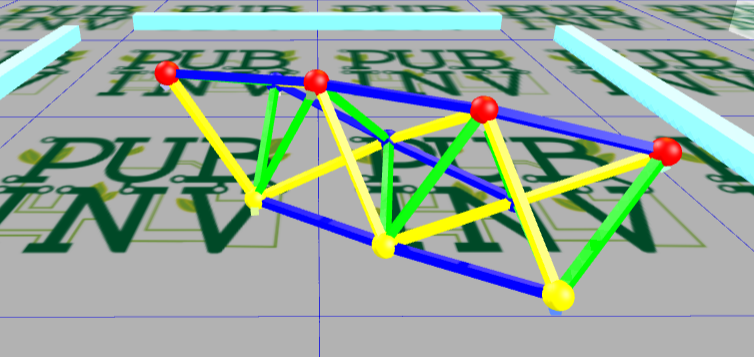
\includegraphics[width=0.4\textwidth]{figures/Tetrahelix1.png}
     \caption{2/3rd Twisted Tetrahelix}
     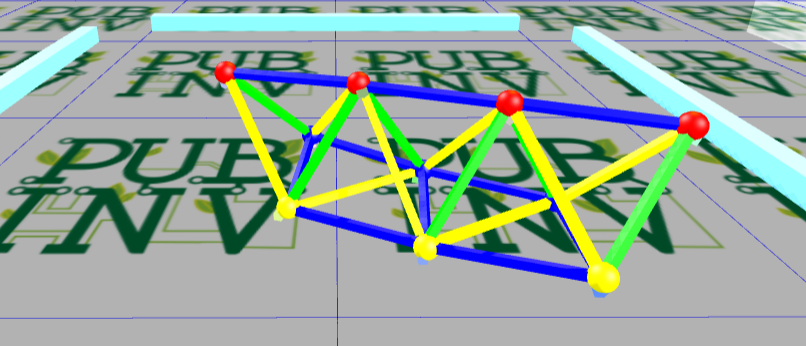
\includegraphics[width=0.4\textwidth]{figures/Tetrahelix2.png}
     \caption{1/3rd Twisted, 2/3rd Untwisted Tetrahelix}
     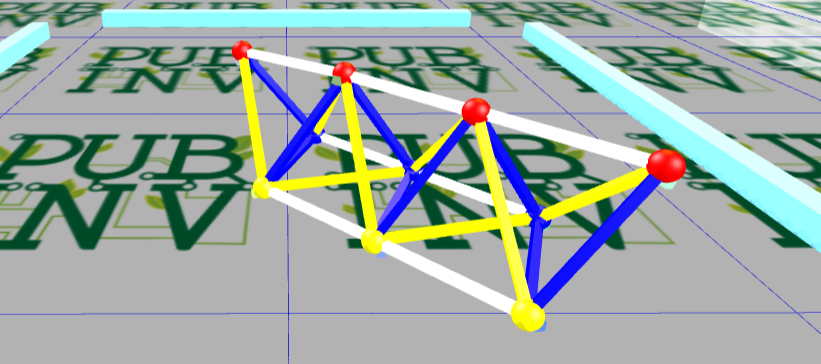
\includegraphics[width=0.4\textwidth]{figures/Tetrahelix3.png}
     \caption{The Equitetrabream: Fully Untwisted Tetrahelix}
\end{figure}

\section{Conclusion}

The BC Helix is the end point of a continuum of tetrahelices, the
other end point being an uncurved tetrahelix with equilateral cross
section, constructed by changing the length of only those members
crossing the outside rails after hopping over the nearest
vertex. Under the condition of miminum maximum length difference of
all members in the system, all such tetrahelices have vertices evenly
spaced along the axis generated by a simple equation.  A mechanical
machine, such as a robot or a variable-geometry truss, that can change
the length of its members, can thus twist and untwist itself by
changing the length of the appropriate members to achieve any point in
the continuum optimally. With a numeric solution, a design may choose
a rotation angle and member lengths to obtain any desired pitch.

\section{Contact and Getting Involved}

The Gluss Project \url{http://pubinv.github.io/gluss/}
is a free-libre, open-source research, hardware, and software project that welcomes volunteers.
It is our goal to organize projects for the benefit of all humanity without seeking profit or intellectual property.
To assist, contact \href{mailto:read.robert@gmail.com}{$<$read.robert@gmail.com$>$}.

\bibliographystyle{IEEEtran}
\bibliography{IEEEabrv,gluss}

\end{document}

TODO:

Clean up d_{opt}.

Produce mini table of pitch vs. \rho?

Improve clarity and precision of proofs.

Solve the chirality problem.

Check every step of my derivation at rho = 0 and the BC values.

Found something.  So now the computation of the optimal radii seems slightly better than what we had before.
We have not, however, proven it to be optimal in the ranges involved, but at least we seem to be computing it correctly.

See if we can accurately compute the derivative of two-hop - one-hop and if it is always negative, meaning that
it is always optimal to set one-hop = 1.  The we have a way to compute one-hope.

Remove the weirdly colored diagram.

Add to the rail angle diagram.

Note that Lamba = 16 almost produces a 2-rail helicoid.

When abs(lambda) > 4, we seem to have marked differences in the parameters. Understand why this is and what is causing it.
(it is possible that positive and negative rho values behave very differently?

Note: Would be really nice to have the GUI show you all computed parameters.

Note: Distance is clearly lower on first computations..

Create working toolkit for desin/exploration.

Improve code that way, use white background, floor.

Figure out if I am computing something wrong.



Try to compute optimal radius within our context. This would let us assert that we have
an ``optimum'' continuum.  Not worth much to an engineer, but valuable.

Review and continue editing, being careful to introduce concepts in the correct order.

On Rail diagram, add a second tetrahedron, and a second rho.



Make YouTube video.


    \section{Old Proofs}
    
We can create the distance between representative nodes as:
\begin{align*}
  \overline{\rm AB}  &= 1 \\        
  \overline{\rm CD}  &= \sqrt{G^2 + r^2(1 + -\cos{2 G \rho})} \\
  \overline{\rm AC}  &= \sqrt{O^2 + r^2(1 + \sin^2{O \rho}  - \cos^2{O \rho})} \\  
  \overline{\rm AC}  &= \sqrt{O^2 + r^2(1 + -\cos{2 O  \rho})} \\
  \overline{\rm BD}  &= \sqrt{P^2 + r^2(1 + -\cos{2 P \rho}))} \\
  \overline{\rm AD}  &= \sqrt{(O+G)^2 + r^2(1 + -\cos{2 (O + G)  \rho})} \\
  \overline{\rm BC}  &= \sqrt{(P+G)^2 + r^2(1 + -\cos{2 (P + G) \rho})} \\      
\end{align*}


Using the cartesian distance formula:
\begin{align*}
  \overline{\rm CD}  &= \sqrt{G^2 + (r\sin{0 \rho} -  r\sin{G \rho})^2 + (r\cos{0 \rho} - r\cos{G \rho})^2} \\
    \overline{\rm CD}  &= \sqrt{G^2 + (0 -  r\sin{G \rho})^2 + (r - r\cos{G \rho})^2} \\
    \overline{\rm CD}  &= \sqrt{G^2 + r^2(\sin{G \rho})^2 + r^2(1 - \cos{G \rho})^2} \\
    \overline{\rm CD}  &= \sqrt{G^2 + r^2(1 + \sin^2{G \rho}  - \cos^2{G \rho})} \\
    \overline{\rm CD}  &= \sqrt{G^2 + r^2(1 + -\cos{2 G \rho})} \\        
\end{align*}
Note: $\sin^2{x \rho}  - \cos^2{x \rho} = -\cos{2 x \rho}$

So, for all O,G,P,
\begin{align*}
  \overline{\rm AB}  &= 1 \\        
  \overline{\rm CD}  &= \sqrt{G^2 + r^2(1 + -\cos{2 G \rho})} \\
  \overline{\rm AC}  &= \sqrt{O^2 + r^2(1 + \sin^2{O \rho}  - \cos^2{O \rho})} \\  
  \overline{\rm AC}  &= \sqrt{O^2 + r^2(1 + -\cos{2 O  \rho})} \\
  \overline{\rm BD}  &= \sqrt{P^2 + r^2(1 + -\cos{2 P \rho}))} \\
  \overline{\rm AD}  &= \sqrt{(O+G)^2 + r^2(1 + -\cos{2 (O + G)  \rho})} \\
  \overline{\rm BC}  &= \sqrt{(P+G)^2 + r^2(1 + -\cos{2 (P + G) \rho})} \\      
\end{align*}




Then we can simplify our distance equations:
\begin{align*}
  \overline{\rm AB}  &= 1 \\        
  \overline{\rm CD}  &= \sqrt{G^2 + r^2(1 + -\cos{2 G \rho})} \\
  \overline{\rm AC} &=   \overline{\rm BD} &= \sqrt{P^2 + r^2(1 + -\cos{2 P \rho}))} \\
  \overline{\rm AC} &=   \overline{\rm BD} &= \sqrt{((1-G)/2)^2 + r^2(1 + -\cos{ \rho (1-G) }))} \\  
  \overline{\rm AD} &=  \overline{\rm BC} &=  \sqrt{((P+G)^2 + r^2(1 + -\cos{2 (P + G) \rho})} \\
  \overline{\rm AD} &=  \overline{\rm BC} &=  \sqrt{((1+ G)/2 )^2 + r^2(1 + -\cos{\rho (1 + G)})} \\        
\end{align*}

When $G = 0$, $\overline{\rm CD} = 0$. Our solution is improved as we
increase $G$ until either $ \overline{\rm CD} = \overline{\rm AC}$, or
the quantity $ \overline{\rm BC} - \overline{\rm CD} $ starts
increasing rather than decreasing (that is, when the derivative is
positive.)



Suppose $\overline{\rm C'D'}$ is the shortest edge. Increasing $G$
thereby improves our mimimum, up until the next shortest edge length,
$\overline{\rm AC}$.  This may increase $\overline{\rm BC}$ and
$\overline{\rm AD}$, but more slowly than $\overline{\rm C'D'}$
is being increased, until $\overline{\rm C'D'} = \overline{\rm AC}$.
Note: This is sketchy, can we show that the derivative of our formula
for CD with respect to $G$ is really higher than $AD$? These
derivatives will depend on $\rho$ slightly, which is exactly right!

\begin{align*}
  \text{rail} &=  1 \\
  \text{one-hop} &= \sqrt{\frac{1}{3}^2 + (\frac{3a}{2\sqrt{3}})^2 + (a/2)^2}\\
\text{one-hop}  &= \sqrt{\frac{1}{9} + a^2} \\
    \text{two-hop} &= \sqrt{\frac{2}{3}^2 + (\frac{3a}{2\sqrt{3}})^2 + (a/2)^2}  \\
\text{two-hop}    &= \sqrt{\frac{4}{9} + a^2}
\end{align*}
Computing the derivative of two-hop - one-hop:
\begin{align*}
 \frac{\partial \text{two-hop} - \text{one-hop}}{a} &= \frac{\partial \sqrt{4/9 + a^2} - \sqrt{1/9 + a^2}}{\partial a} \\
  \frac{\partial \text{two-hop} - \text{one-hop}}{a} &= \frac{a}{\sqrt{a^2 + 4/9}} - \frac{a}{\sqrt{ a^2 + 1/9}} 
\end{align*}

  
Now basic components of the helix, which are the radius $r$, the rate of rotation, and the rate of
axial growth can all be linearly interpolated with a parameter $\lambda$ between their high values (for the BC helix)
and low values (for the equitetrabeam):

\begin{align*}
r_{\lambda}  &=  \lvert \lambda \rvert \cdot (\frac{3 \sqrt{3}}{10}  - \sqrt{\frac{8}{27}}) + \sqrt{\frac{8}{27}}  \\
d_{\lambda} &=   \lvert \lambda \rvert \cdot (3 \sqrt{10} - 1) + 1 \\
\phi_{\lambda} &=  \lambda \cdot \rho_{bc}  + 0
\end{align*}
to create a formula that generates a continuum of tetrahedral structures:

\[
H_{continuum}(n,c,\lambda) =
\left [
  \begin{tabular}{c}
   $ r_{\lambda} \cos(\phi_{\lambda} \kappa + c 2 \pi /3) $\\
   $ r_{\lambda}  \sin(\phi_{\lambda} \kappa + c 2 \pi /3) $\\
   $ d_{\lambda} \kappa $
  \end{tabular}
  \right ],
\text{where:}
  \begin{tabular}{c}
    $\kappa = n + c/3$ \\
    $ r_{opt} =  \text{is used : \eqref{eqrhoopt}} $ \\    
    $ \phi_{\lambda} =  \lambda \rho_{bc}  + 0 $\\
    $\rho_{bc} = (3 \theta - 2 \pi)$ \\
   $ \theta = \arccos(-2/3) $
  \end{tabular}      
  \]



  Consider any tetrahelix in which the axes of the helices are parallel
to $z$ but not coincident, but in which all vertices lie on or outside
a cylinder of radius $r$ centered on the $z$ axis.
Since all three rails have the same rail length, no matter how we
move the rails in the $xy$ plane if we shorten the $xy$ distance between
vertices we shorten the total distance.
Consider the projection along the $z$ axis of all vertices and non-rail edges into the $xy$ plane, which will be
a figure of dots and connecting segments in the $xy$ plane. The convex
hull for any one helix projection will be a circle (if its pitch is
irrational) or an polygon if rational, or a point if the helix has
zero curvature. Each of these figures by definitions lies outside the
circle of radius $r$ in the $xy$ plane.
It is easiest to consider helices of zero curvature which only have one point
as a special case. 
For one rail consider a point in this projected figure furthest from the midpoint of the
the two rails. The lengths to the furthest point on the other two rails will
be decreased by moving the axis of that rail closer to the midpoint of the
other two.
One of these segements
will be longer and will be made shorter by moving that helix closer to
the midpoint of the other two in the $xy$ plane. Even if the rail
angle is $\pi$, there will be two vertices for each rail, each of
which is connected to both vertices of the other two rails. At lesast
one of these lines is a longest line which will be made shorter by
moving that helix in the $xy$ plane closer to the midpoint of the
other two.

For the special case of degenerate helix where we do not know the angle
of the points from the axis, we can see that we minimize the maximum lengths
when the projected vertices form an equilateral triangle around the $z$ axis at
length $6r/\sqrt{3}$.
This is a equivalent to some set of helices which do have their axes on
the $z$ axis, so without loss of generality we treat these degenerate
helices as if they have their axis at the $z$-axis.

So any any optimal tetrahelix with a rail-angle of greater than $0$,
that is, with any curvature, will have conincident axes, or are indistinguishable
from such a set.





Possible addtional refrerences and submissions:

Journal of applied geometry seems like a good fit:

http://epubs.siam.org/toc/sjaabq/1/1

According to there editorial board, they welcome mathematcal software and
online resources such as I provie.

This one has a nice editing structure: Metric Geometry is a nice subset:

http://discreteanalysisjournal.com/for-authors

  
http://bit-player.org/2013/tetrahedra-with-a-twist

This is unrelated, but well worth reading:

https://arxiv.org/pdf/1702.06388.pdf
